\documentclass[acmtog]{acmart}
\usepackage{graphicx}
\usepackage{subfigure}
% Title portion
\title{Assignment 5 - Volume Rendering Using Ray-casting} 
\author{Name:\quad Su'an Xia  \\ student number:\quad 18047482
	\\email:\quad xiasa@shanghaitech.edu.cn}

% Document starts
\begin{document}
\maketitle

\vspace*{2 ex}


\section{Introduction}
\subsection{pre-processing}
Requirement: Compute the gradient of the volume data (density).

\vspace*{1 ex}
\subsection{Sampler}
Requirement: Sample a data point along the ray direction.

\vspace*{1 ex}
\subsection{Interpolator}
Requirement: Interpolate data from nearby grid points to decide the value of sampled point.

\subsection{Classifier}
Requirement: Classifier decides its color and opacity based on its values. .

\subsection{Compositor}
Requirement: Collect and integrate the color and opacity of sampled point one by one.

\subsection{Render}
Requirement: Assembles all the components above and outputs the resulting image..

\vspace*{2 ex}
\section{IMPLEMENTATION DETAILS}
\subsection{pre-processing}
In volume.cpp, we need to complete the function 'void Volume::computeGradients()'.
\\Use central difference to compute the gradients.
\\For boundary points, the gradient is the same as the nearest inner point.
\\For inner points, calculate the corresponding difference in density along dx,dy,dz direction.

\vspace*{1 ex}
\subsection{Sampler}
In renderer.cpp, we should implement the sample when we assemble all the steps.
\\A fixed step is ok.

\subsection{Interpolator}
In interpolator.h, we need to complete the class 'TrilinearInterpolator'
\\Given the volex,we can easily calculate the density and gradient by formular.

\subsection{Classifier}
In classifier.h, we need to complete the function 'transfere()'.
\\We use 'tinycolormap' to map a density to a color.
\\The we use Phong shading model to render.
\\Get the final color with considering the effect of gradient.
\\Get the transparency.

\subsection{Compositor}
In compositor.cpp, we need to complete the function 'compositeFrontToBack'.
\\$C_{dst} = C_{dst} + (1-\alpha_{dst})C_{src}$.
\\$\alpha_{dst} = \alpha_{dst} + (1-\alpha_{dst})\alpha_{src}$.

\subsection{Render}
In renderer.cpp, we need to complete the function 'renderFrontToBack()'.
\\Assemble all the functions in the following sequences:
\\Sample, Interpolator, Classfier, Compositor.

\vspace*{2 ex}

\section{Results}

\begin{figure}[h]
\centering
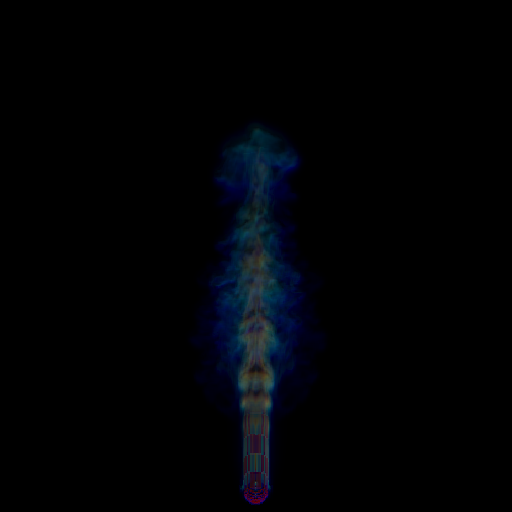
\includegraphics[width=6cm,height=8cm]{Near+2.png}
\caption{Nearest,2*dx}
\end{figure}

\begin{figure}[h]
	\centering
	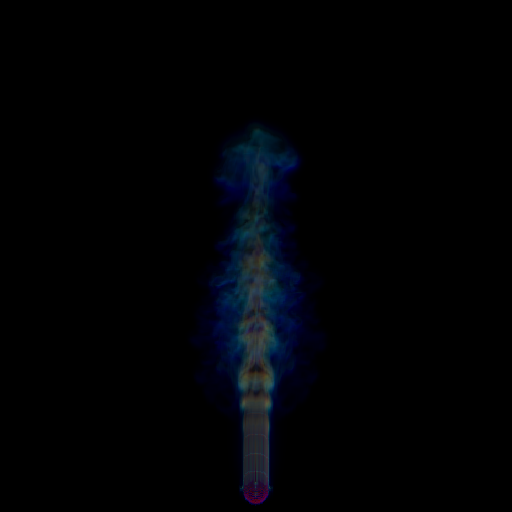
\includegraphics[width=6cm,height=8cm]{Near+1.png}
	\caption{Nearest, 1*dx}
\end{figure}
\begin{figure}[h]
	\centering
	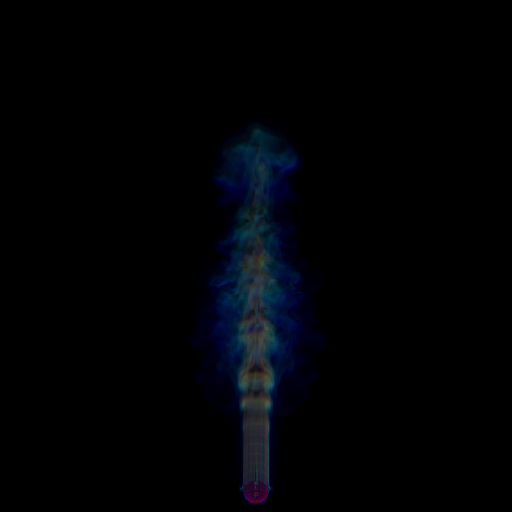
\includegraphics[width=6cm,height=8cm]{Near+half.png}
	\caption{Nearest, 0.5*dx}
\end{figure}
\begin{figure}[h]
	\centering
	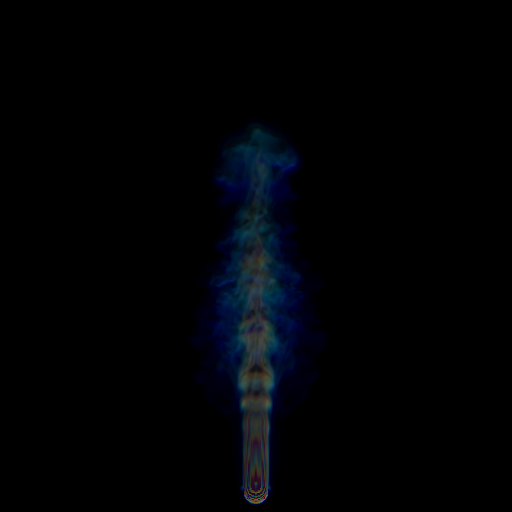
\includegraphics[width=6cm,height=8cm]{Trilinear+2.png}
	\caption{Trilinear, 2*dx}
\end{figure}
\begin{figure}[h]
	\centering
	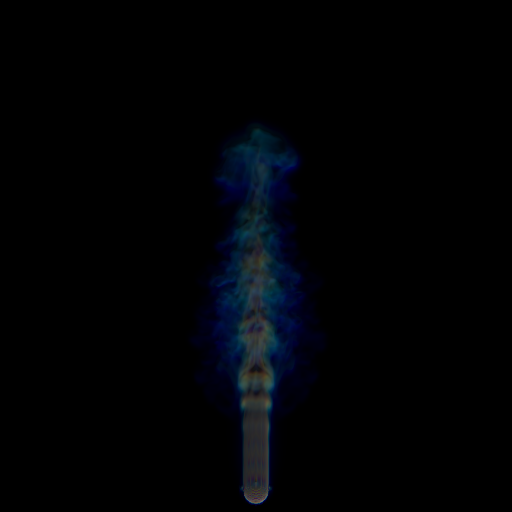
\includegraphics[width=6cm,height=8cm]{Trilinear+1.png}
	\caption{Trilinear, 1*dx}
\end{figure}
\begin{figure}[h]
	\centering
	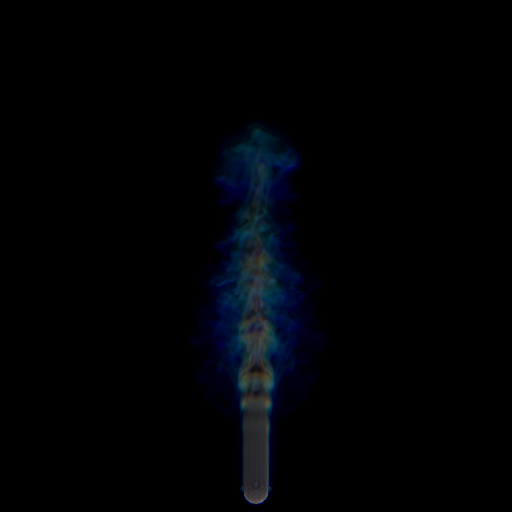
\includegraphics[width=6cm,height=8cm]{Trilinear+half.png}
	\caption{Trilinear, 0.5*dx}
\end{figure}
\begin{figure}[h]
	\centering
	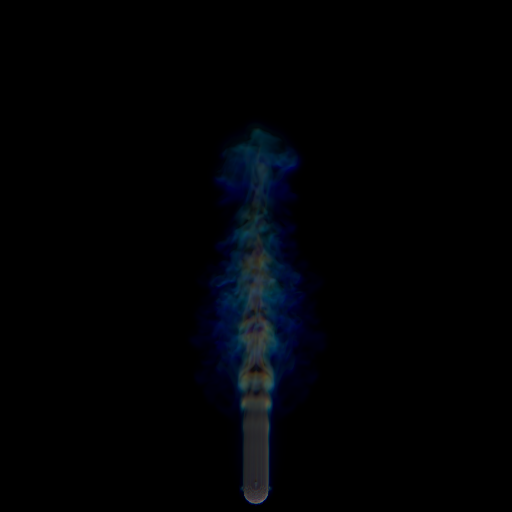
\includegraphics[width=6cm,height=8cm]{Trilinear+120.png}
	\caption{Trilinear, dx/3}
\end{figure}

\end{document}
